%%%% ijcai18.tex

\typeout{IJCAI-18 Instructions for Authors}

% These are the instructions for authors for IJCAI-18.
% They are the same as the ones for IJCAI-11 with superficical wording
%   changes only.

\documentclass{article}
\pdfpagewidth=8.5in
\pdfpageheight=11in
% The file ijcai18.sty is the style file for IJCAI-18 (same as ijcai08.sty).
\usepackage{ijcai18}

% Use the postscript times font!
\usepackage{times}
\usepackage{xcolor}
\usepackage{soul}
\usepackage[utf8]{inputenc}
\usepackage[small]{caption}

\usepackage{amsfonts}
\usepackage{amsmath} % assumes amsmath package installed
\usepackage{amssymb}  % assumes amsmath package installed
\usepackage{amsthm} %\usepackage{graphicx}
\usepackage{graphics} % for pdf, bitmapped graphics files
\usepackage{mathptmx} % assumes new font selection scheme installed
\usepackage{url}
\usepackage{rotating}
\usepackage{subfigure}
\usepackage{enumitem}
\usepackage[linesnumbered,ruled,lined]{algorithm2e}

% the following package is optional:
%\usepackage{latexsym} 

% Following comment is from ijcai97-submit.tex:
% The preparation of these files was supported by Schlumberger Palo Alto
% Research, AT\&T Bell Laboratories, and Morgan Kaufmann Publishers.
% Shirley Jowell, of Morgan Kaufmann Publishers, and Peter F.
% Patel-Schneider, of AT\&T Bell Laboratories collaborated on their
% preparation.

% These instructions can be modified and used in other conferences as long
% as credit to the authors and supporting agencies is retained, this notice
% is not changed, and further modification or reuse is not restricted.
% Neither Shirley Jowell nor Peter F. Patel-Schneider can be listed as
% contacts for providing assistance without their prior permission.

% To use for other conferences, change references to files and the
% conference appropriate and use other authors, contacts, publishers, and
% organizations.
% Also change the deadline and address for returning papers and the length and
% page charge instructions.
% Put where the files are available in the appropriate places.


\setcounter{secnumdepth}{2}  

%Macros
\def\no{\; {not} \;}
%\def\no{\textit{ not }}x
\def\myif{\texttt{:-}}
\newcommand{\defeq}{:=}
\newcommand{\stt}[1]{{\small\texttt{#1}}}

\newtheorem{example2}{\bf Example}
\newtheorem{execexample}{\bf Execution Example}
\newtheorem{example3}{\bf Example Domain}
\newtheorem{definition}{Definition}
\newtheorem{proposition}{Proposition}
\newtheorem{lemma}{Lemma}
\newcommand{\rif}{\stackrel{\,\,+}{\leftarrow}}
%end of Macros

\long\def\comment#1{{\bf **#1**}}
\long\def\commentm#1{{\bf **Mohan: #1**}}
\long\def\commentb#1{{\bf **Ben: #1**}}

\newenvironment{s_itemize}{\begin{list}{$\bullet$}
{\setlength{\rightmargin}{0em}
\setlength{\itemsep}{0em}
\setlength{\topsep}{0em}
\setlength{\parsep}{0em}}}{\end{list}}

\newenvironment{small_ind_s_itemize}{\begin{list}{$\bullet$}
{\setlength{\rightmargin}{0em}
\setlength{\leftmargin}{1em}
\setlength{\itemsep}{0em}
\setlength{\topsep}{0em}
\setlength{\parsep}{0em}}}{\end{list}}

\newcounter{ctr}
\newenvironment{s_enumerate}{\begin{list}{\thectr.}
{\usecounter{ctr}
\setlength{\rightmargin}{0.3cm}
\setlength{\leftmargin}{0.3cm}
\setlength{\itemsep}{0em}
\setlength{\topsep}{0em}
\setlength{\itemindent}{0.5cm}
\setlength{\parsep}{0em}}}{\end{list}}

\newenvironment{small_ind_enumerate}{\begin{list}{\thectr.}
{\usecounter{ctr}
\setlength{\rightmargin}{\rightmargin}
\setlength{\leftmargin}{0.3em}
\setlength{\itemsep}{\itemsep}
\setlength{\topsep}{\topsep}
%\setlength{\itemindent}{0.5cm}
\setlength{\parsep}{\parsep}}}{\end{list}}


\title{Knowledge Representation and Interactive Learning of \\
Domain Knowledge for Human-Agent Interaction}

% \author{ Mohan Sridharan \and Ben Meadows \\ 
%   Department of Electrical and Computer Engineering\\
%   The University of Auckland, Auckland 1023, NZ \\
%   \{m.sridharan@auckland.ac.nz, bmea011@aucklanduni.ac.nz\}}


\begin{document}
\maketitle

\begin{abstract}
  This paper describes an architecture that enables representation of,
  reasoning with, and interactive learning of domain knowledge in the
  context of human-robot collaboration.  Specifically, the robot
  represents and reasons with incomplete domain knowledge using Answer
  Set Prolog, a declarative programming paradigm. ASP-based reasoning
  is used to identify gaps in existing knowledge and guide the
  interactive learning of axioms corresponding to knowledge of the
  preconditions and effects of actions, and of previously unknown
  actions and affordances.  This learning uses observations obtained
  through active exploration, reactive action execution, and verbal
  feedback from humans, and the learned axioms are included in the
  knowledge based for subsequent reasoning.  The architecture is
  evaluated in the context of a simulated robot assisting humans in an
  indoor domain.
\end{abstract}







%%%%%---------------------------------------------------------------------------------
%%%%%---------------------------------------------------------------------------------
\section{Introduction}
\label{sec:introduction}
Consider one or more robots\footnote{We use the terms ``robot'', and
  ``learner'' interchangeably.} assisting humans in an office domain.
Each such robot will be assigned tasks of varying complexity in a
dynamic environment, e.g., find and deliver particular objects to
particular places (or people), or guide people to particular
locations. The robot will find it challenging to perform these tasks
without considerable domain knowledge and/or guidance.  This includes
commonsense knowledge, especially default knowledge that is true in
all but a few exceptional circumstances, e.g., ``plates are usually in
the kitchen, but used plates may also be on the dining table''. It
also includes knowledge of action preconditions and effects, and
affordances. At the same time, it will be difficult for human
participants to possess the time and expertise to provide
comprehensive information about the domain or elaborate feedback. To
truly assist humans, robots will thus need the ability to reason with
incomplete domain knowledge, and to revise this knowledge over time;
these are open problems in robotics and AI.

The challenges described above are offset by the robot's ability to
learn interactively using observations obtained in response to active
exploration or reactive action execution. The architecture described
in this paper seeks to support such interactive learning in
conjunction with the ability to reason with incomplete domain
knowledge. The architecture is based on the following tenets:
\begin{s_itemize}
\item Knowledge elements include symbolic content encoding object
  constants, relations representing domain attributes and actions at
  different levels of abstraction, and axioms composed of these
  relations.

\item Knowledge elements are revised non-monotonically by reasoning
  with the existing knowledge and (a history of) observed action
  outcomes.

\item Effects of action execution may be immediate or delayed, and
  action capabilities (i.e., ``affordances'') are defined jointly over
  the attributes of agents and objects in the context of particular
  actions.

\item Learning is coupled with interaction, revising the relative
  value of state-action combinations using observations of active
  exploration and reactive action execution.
\end{s_itemize}
This paper implements these tenets by combining the complementary
strengths of declarative programming, probabilistic reasoning, and
relational learning through induction and reinforcement. To focus on
the interplay between reasoning and learning, we abstract away some
levels of representation, including the probabilistic modeling of
uncertainty in perception and actuation---highly probable beliefs are
elevated to logic statements associated with complete certainty. We
also assume that the domain may have multiple robots with identical
capabilities, which cannot communicate with each other. We described
the following characteristics of our architecture:
\begin{s_itemize}
\item Incomplete domain knowledge described in an action language is
  translated into a relational representation in Answer Set Prolog
  (ASP) for inference, planning and diagnostics. ASP-based reasoning
  also automatically limits interactive learning to the relevant part
  of the domain.

\item Previously unknown actions' names, preconditions, effects, and
  objects over which they operate, along with associated affordances,
  are learned using decision-tree induction and relational
  reinforcement learning based on observations of active exploration,
  reactive action execution, and verbal cues from humans.
\end{s_itemize}
These characteristics are illustrated in the context of a simulated
robot interacting with and assisting humans by moving desired objects
to particular people or locations. We first describe the proposed
architecture and algorithm (Section~\ref{sec:arch}), followed by the
results of experimental evaluation (Section~\ref{sec:exp}). Then,
Section~\ref{sec:relwork} reviews some related work, followed by a
description of conclusions and future work
(Section~\ref{sec:conclusions}).


%%%%%---------------------------------------------------------------------------------
%%%%%---------------------------------------------------------------------------------
\section{Proposed Architecture}
\label{sec:arch}

\begin{figure}[tb]
  \begin{center}
    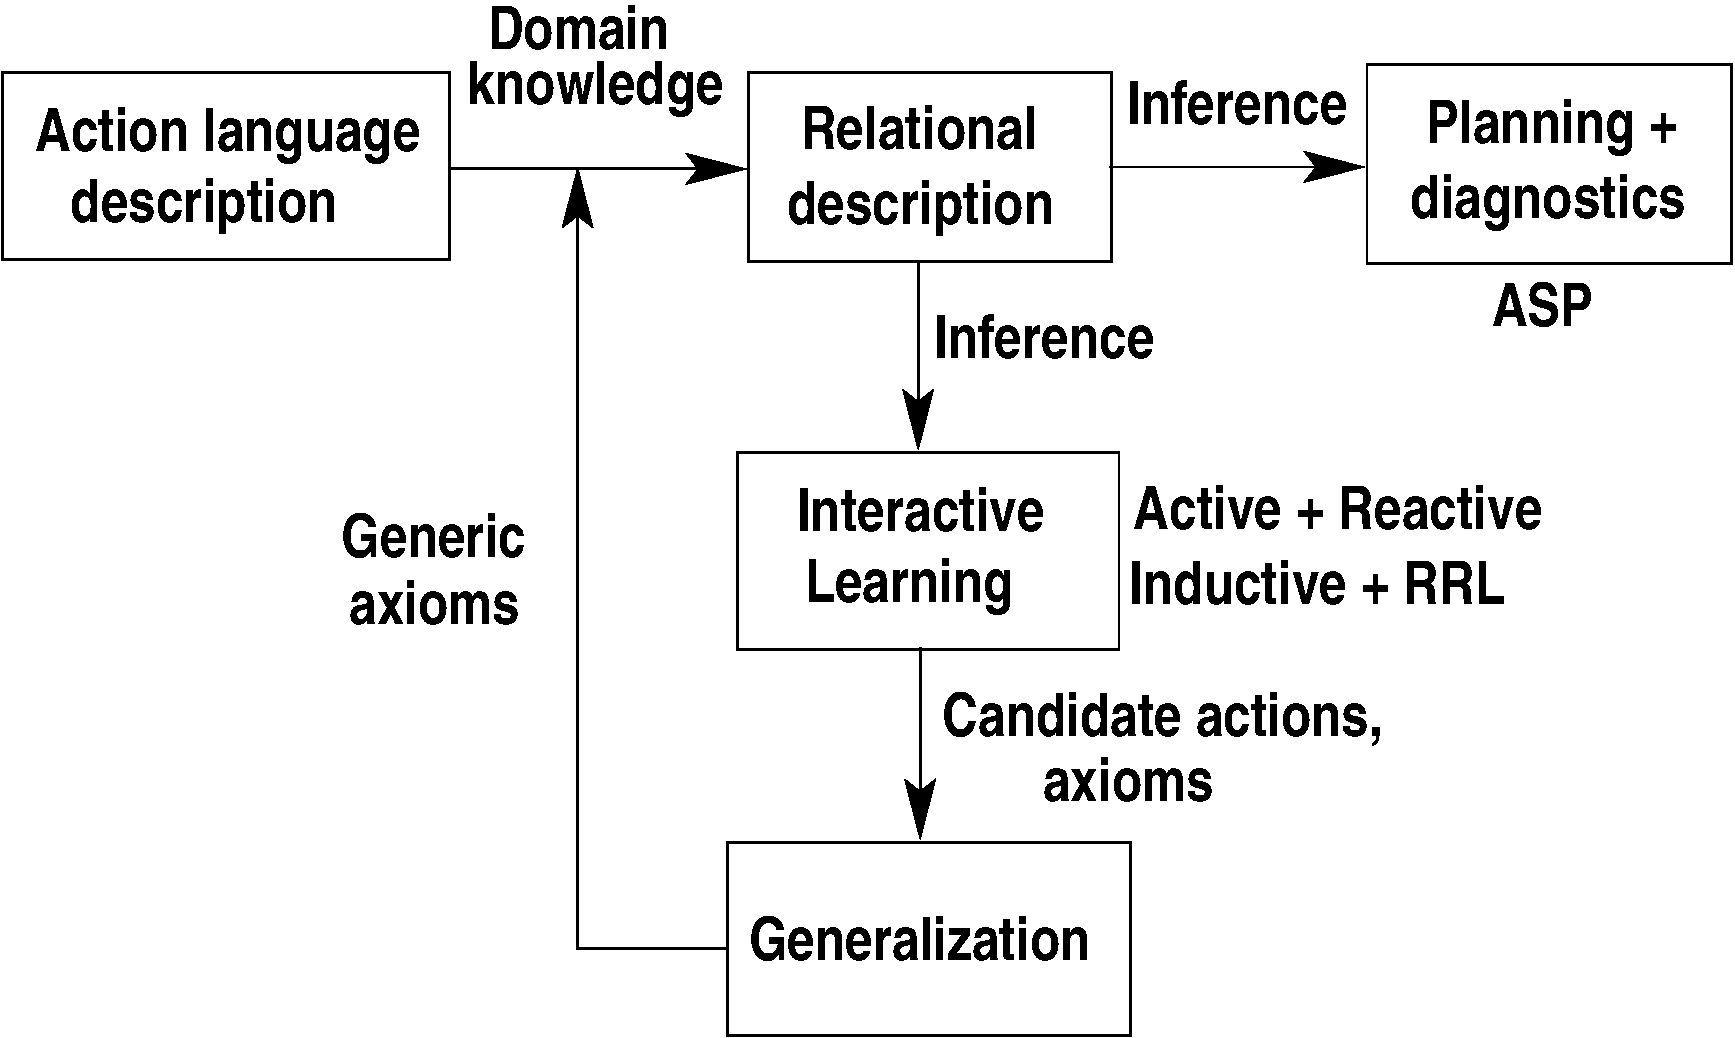
\includegraphics[width=\columnwidth]{./Images/overview}
  \end{center}
  %\vspace{-1.5em}
  \caption{Architecture combines declarative programming and
    interactive learning for reasoning with and learning domain
    knowledge.}
  \label{fig:overview}
  %\vspace{-1.5em}
\end{figure}

Figure~\ref{fig:overview} presents an overview of the proposed
architecture. Incomplete domain knowledge is encoded in an action
language and used with knowledge of initial state to construct a
relational representation. As stated earlier, we abstract away the
reasoning at different levels of abstraction and probabilistic
reasoning of uncertainty, to focus on the interplay between reasoning
and interactive learning. The relation representation is thus
translated to an ASP program that is solved for planning and
diagnostics. Reasoning with the ASP program is also used to guide the
interactive learning of domain knowledge. Here we focus on learning
about actions, affordances, and the preconditions and effects of
actions, using observations obtained from active exploration, reactive
execution, and human input. The learned knowledge is added to the ASP
program and used for subsequent reasoning. We illustrate the
architecture's capabilities using the following simulated domain.

\begin{example2}\label{ex:illus-example}[Robot Assistant (RA) Domain]
  {\rm Our illustrative domain has a simulated robot/learner finding,
    labeling and delivering objects to people or places (office,
    kitchen, library, workshop) in an office building. Each place
    (i.e., room) has one or more instances of objects such as $desk$,
    $book$, $cup$ and $computer$. Human(s) in each room may have a
    different $role$ (engineer, manager, salesperson). Objects are
    characterized by $weight$ ($\{heavy, light\}$), $surface$
    ($\{brittle, hard\}$), $status$ ($\{intact, damaged\}$), and
    $labeled$ ($\{true, false\}$).  The robot's arm is characterized
    by $type$ ($\{electromagnetic, pneumatic\}$). The actions
    available to the robot include $pickup$, $putdown$, $move$,
    $label$, and $serve$, but it may not (for instance) know that it
    can label objects or serve them to specific people.  Furthermore,
    it does not know various axioms associated with $serve$ action,
    including:
    \begin{itemize}
    \item A pneumatic arm cannot be used to serve a brittle object.
    \item Serving an object to a salesperson causes it to be labeled.
    \end{itemize}
    Similarly, unknown axioms for the $label$ action include:
    \begin{itemize}
    \item An object with brittle surface cannot be labeled unless the
      robot has an electromagnetic arm.
    \item Labeling a light object with a pneumatic arm causes it to be
      damaged.
    \end{itemize}
    There are one or more other robots with identical capabilities,
    but they cannot communicate with the learner. Human participants
    (if any) and the learner can observe these other robots, and
    humans can provide verbal cues describing the activities of the
    other robots, e.g., ``Robot labeled the hard, hefty item''. The
    objective is for the learner to learn about the previously unknown
    actions and axioms governing domain dynamics.

    Note that this domain can become considerably complex as the
    number of objects and their attributes increases. For example, in
    one scenario that we used in our experiments, there were $\approx
    18000$ static attribute combinations and $\approx 11 million$
    physical object configurations.  }
\end{example2}



%%%%%---------------------------------------------------------------------------------
\subsection{Knowledge Representation and Reasoning}
\label{sec:arch-asp}
Action languages are formal models of parts of natural language that
are used for describing action effects. We use action language
$AL_d$~\cite{gelfond:ANCL13} to describe the transition diagrams of
our domains. $AL_d$ has a sorted signature with three $sorts$: (i)
\emph{statics}, i.e., domain properties whose truth values cannot be
changed by actions; (ii) \emph{fluents}, i.e., domain properties whose
truth values can be changed by actions; and (iii) and \emph{actions}.
\emph{Basic} fluents obey laws of inertia and are changed directly by
actions, whereas \emph{defined} fluents do not obey inertial laws and
are not changed directly by actions. A domain property \emph{p} or its
negation $\lnot p$ is a domain \emph{literal}. $AL_d$ allows three
types of statements: causal law, state constraint, and executability
condition, examples of which are provided later in this section.
% \begin{align*}
%   &a~~\mathbf{causes}~~l_b~~\mathbf{if}~p_0,\ldots,p_m~\textrm{(Causal
%     law)} \\ \nonumber
%   &l~~\mathbf{if}~~p_0,\ldots,p_m~~~~~~\textrm{(State
%     constraint)}\\\nonumber
%   &\mathbf{impossible}~~a_0,\ldots,a_k~~\mathbf{if}~~p_0,\ldots,p_m
%   ~\textrm{(Executability condition)}
% \end{align*}
% where $a$ is an action, $l$ is a literal, $l_b$ is a basic literal,
% and $p_0,\ldots,p_m$ are domain literals.


%%%%%-------------------------------------------------------------------
\subsubsection{Domain Representation: Signature and Axioms}
The domain representation consists of system description
$\mathcal{D}$, a collection of statements of $AL_d$, and history
$\mathcal{H}$. $\mathcal{D}$ has a sorted signature $\Sigma$ and
axioms that describe the transition diagram $\tau$. $\Sigma$ defines
the basic sorts, and domain properties and actions. For instance,
basic sorts of the RA domain include $place$, $robot$, $role$, $book$,
$computer$, $weight$, $status$, $type$ etc.  Sorts that are subsorts
of other sorts, e.g., $cup$ and $book$ are subsorts of $object$, are
arranged hierarchically.  $\Sigma$ also includes ground instances of
sorts, e.g., $rob_1$ of sort $robot$, $\{office, workshop, kitchen,
library\}$ of sort $place$, and $\{engineer, manager, salesperson\}$
of sort $role$, and sort $step$ for temporal reasoning.

Domain properties and actions are described in terms of the sorts of
their arguments. The RA domain includes fluents such as $loc(entity,
place)$, the location of the robot and objects, with the location of
humans and other robots (if any) modeled as a defined fluent whose
value is obtained from other (external) sensors; and $in\_hand(robot,
object)$, which denotes whether a particular object is in the robot's
hand. Static attributes of the domain include $arm\_type(robot,
type)$, $obj\_weight(object, weight)$ etc. Actions available to the
robot include $move(robot, place)$, $pickup(robot, object)$,
$putdown(robot, object)$, $serve(robot, object, person)$, and
$label(robot, object)$.  Furthermore, the relation $holds(fluent,
step)$ implies that a particular fluent holds true at a particular
timestep.

\smallskip
\noindent
For the RA domain, $\mathcal{D}$ includes axioms such as:
\begin{align*}
  &move(rob_1, L)~~\mathbf{causes}~~loc(rob_1, L) \\
%  &pickup(rob_1, O)~~\mathbf{causes}~~in\_hand(rob_1, O) \\
  &serve(rob_1, O, P)~~\mathbf{causes}~~in\_hand(P, O)\\
  &\neg loc(E, L_2)~~\mathbf{if}~~loc(E, L_1),~ L_1\neq L_2 \\
  &loc(O, L)~~\mathbf{if}~~ loc(rob_1, L),~in\_hand(rob_1, O)\\
  &\mathbf{impossible}~~pickup(rob_1, O)~~\mathbf{if}~~loc(rob_1,
  L_1), loc(O, L_2),\\ 
  &\qquad~~~~~~~~~~~~~~~~~~~~~~~~~~~~~~~~~~~~~~~~~~~~~L_1\neq L_2
\end{align*}

The domain representation includes history $\mathcal{H}$, which (for a
dynamic domain) is usually a record of fluents observed to be true or
false at a time step, i.e., $obs(fluent, boolean, step)$, and the
occurrence of an action at a time step, i.e., $hpd(action,step)$. Our
model of history expands this notion to allow the representation of
defaults describing the values of fluents in their initial states. For
instance, we can encode ``food is usually in the pantry'', and
exceptions, e.g., ``fruits are in the dining room''.


%%%%%-------------------------------------------------------------------
\subsubsection{Domain Representation: Affordances} 
Recall that we define affordances as relations between attributes of
robot(s) and object(s) in the context of particular actions. Negative
(i.e., forbidding or dis-) affordances describe unsuitable
combinations of objects, robots, and actions. Positive affordances
describe permissible uses of objects in actions by agents, including
exceptions to executability conditions that may (normally) prevent the
use of the corresponding action during planning. We represent
affordances in a distributed manner, as follows:
\begin{align*}
  \mathbf{impossible}~~ A &~~\mathbf{if}~~ af\!\!f\_forbids(ID,
  A)\\
  af\!\!f\_forbids(id_i, A) &~~\mathbf{if}~~ \ldots\\
  \mathbf{impossible}~~ A &~~\mathbf{if}~~
  \ldots,~~not~af\!\!f\_permits(ID, A)\\
  af\!\!f\_permits(id_j, A)&~~\mathbf{if}~~ \ldots
\end{align*}
The first two statements say that action $A$ cannot occur if it is not
afforded, and specify the conditions (i.e., attributes of robot and
object) under which the action is not afforded. The last two
statements say that an action $A$ that is not considered during
planning due to a particular executability condition may have a
positive affordance as an exception, and specified the definition of
the positive affordance. Notice that each action can have one or more
positive or negative affordances indexed by the ``id''s. % For instance:
% %\vspace{-0.3em}
% \begin{align*}
%   \mathbf{impossible}~~label(rob_1, Ob) ~~&\mathbf{if}~~ obj\_surface(Ob, brittle), \\ &  not~af\!\!f\_permits(ID, label(rob_1, Ob))\\
%   af\!\!f\_permits(id_1, label(rob_1,
%   Ob))~~&\mathbf{if}~~arm\_type(rob_1, electromagnetic),\\
%   &obj\_surface(Ob, brittle)
% \end{align*}
% where a brittle object cannot usually be labeled, but an
% electromagnetic arm and a brittle object jointly afford labeling. 
This distributed representation of affordances (and knowledge)
improves generalization, and can simplify inference and information
reuse.

% For instance, if the robot in the RA domain knows that a weak arm
% cannot pick up a heavy object, the following statements will be
% included in the ASP program:
% \begin{align*}
%   forbidding\_af\!\!f(id1, pick&up(R, O)) \\
%   fails(id1, pickup(R, O))~&\leftarrow \\ not~& weight(O, heavy)\\
%   fails(id1, pickup(R, O))~&\leftarrow \\ not~& armstrength(R, weak)
% \end{align*}

%%%%%-------------------------------------------------------------------
\subsubsection{ASP-based inference}
The domain representation is translated into a program
$\Pi(\mathcal{D}, \mathcal{H})$ in CR-Prolog\footnote{We use the terms
  ``ASP'' and ``CR-Prolog'' interchangeably.}, a variant of ASP that
incorporates consistency restoring (CR)
rules~\cite{balduccini:aaaisymp03}. ASP is based on stable model
semantics, and supports \emph{default negation} and \emph{epistemic
  disjunction}, e.g., unlike ``$\lnot a$'' that states \emph{a is
  believed to be false}, ``$not~a$'' only implies \emph{a is not
  believed to be true}, and unlike ``$p~\lor\,\,\lnot p$'' in
propositional logic, ``$p~or~\lnot p$'' is not tautologous.  ASP can
represent recursive definitions, defaults, causal relations, and
constructs that are difficult to express in classical logic
formalisms. $\Pi$ consists of causal laws of $\mathcal{D}$, inertia
axioms, closed world assumption for defined fluents, reality checks,
and observations, actions, and defaults recorded in $\mathcal{H}$.
Every default is turned into an ASP rule and a CR rule that allows the
robot to assume, under exceptional circumstances, that the default's
conclusion is false, so as to restore program consistency. Although
not discussed here, $\Pi$ also includes relations and axioms for
diagnostics. The ground literals in an \emph{answer set} obtained by
solving $\Pi$ represent beliefs of an agent associated with $\Pi$.
Algorithms for computing the entailment, and for inference, planning
and diagnostics, reduce these tasks to computing answer sets of
CR-Prolog programs.

In complex, dynamic domains, the robot's knowledge of the domain is
likely to be incomplete, or it may become incorrect over time (e.g.,
affordances may change due to wear and tear). The plans created using
this knowledge may (i) not find valid plans; (ii) find suboptimal
plans; or (iii) provide plans that when executed provide unintended
outcomes. In the illustrative domain, consider a scenario in which the
robot (that is in the $kitchen$) is to deliver the robotics textbook
$bk_1$ to the $of\!\!fice$. The plan, based on the default knowledge
about the location of books ($library$) includes $move(rob_1,
library)$, $pickup(rob_1, bk_1)$, $move(rob_1, of\!\!fice)$, and
$putdown(rob_1, bk_1)$. The robot expects this plan to succeed, but it
may not be able to pick the book up because the robot has an
electromagnetic arm that (unknown to the robot) cannot be used to pick
up the heavy book. In this paper, we focus on learning such previously
unknown domain knowledge through interactive learning.


%%%%%---------------------------------------------------------------------------------
\subsection{Interactive Learning}
\label{sec:arch-learn}
In our architecture, the existing action model can be revised by
learning previously unknown actions, and axioms corresponding to
executability conditions, causal laws, and affordances. Obtaining
labeled samples to learn this knowledge will be difficult in complex
domains, and access to humans may be limited. Also, recall that the
effects of actions may be observed immediately or after a delay, i.e.,
observations may be due to one or more past states and actions.  We
thus enable the robot to interactively acquire labeled samples.  Since
running many trials on a robot to learn generic action descriptions
and axioms may be intractable, we use two schemes: (i) active learning
from verbal cues provided by humans; (ii) relational reinforcement
learning based on observations obtained through active exploration or
reactive action execution. We describe these two schemes below.
% ways. The discovery of positive (i.e., enabling) affordances may
% require the robot to actively explore new object-action
% combinations, including actions expected to fail.  Negative (i.e.,
% forbidding) affordances, which we focus on here, are usually found
% when the unexpected transition observed after executing a plan step
% is considered to imply that the action is inappropriate given the
% object and agent involved. To model the relationships that led to
% this transition, our architecture explores the space of relevant
% transitions, produces candidate relations and axioms corresponding
% to affordances, generalizes across these candidates, validates the
% most likely candidates, and adds them to the system description, as
% described below.

%%%%%-------------------------------------------------------------------
\subsubsection{Learning from Human Interaction}
Recall that the verbal cues provided by a human describe the observed
actions/behaviors of other robots in the domain. To learn from these,
we make the following assumptions:
\begin{s_itemize}
\item Cues describe behavior of robots that have the same capabilities
  as the learner;
\item The learner can generate logic statements corresponding to
  attributes of robot(s) or object(s) involved in the observed action;
\item Humans provide correct descriptions of one observed action or
  activity at a time.
\end{s_itemize}
These assumptions are reasonable for many robotics domains, and result
in simple interaction with humans.

The learner solicits human input when available and receives a
transcribed verbal description of an action and observations of the
action's consequences. For example, the learner may receive as input
``The robot is labeling the fairly big textbook.'' and
[\textit{labelled(book1, true)}]. This information is passed on to a
part-of-speech (POS) tagger---we use the Stanford log-linear POS
tagger~\cite{toutanova:hlt-naacl03}, employing a left, second-order
sequence information model to determine each word's appropriate POS
tag and append it. For the input string considered above, the output
is a string such as ``The\_DT robot\_NN is\_VBZ labeling\_VBG the\_DT
fairly\_RB big\_JJ textbook\_NN''. Here the tags represent parts of
speech, e.g., ``VB'' for verb, ``NN'' is for noun, etc. The learner
transforms this string to
% ((``english-left3words-distsim.tagger" specifically))
$<$word, POS$>$ pairs. It then transforms the sentence's verb into
first person present tense using rules generated from a lemma
list~\cite{lemma-txt} and WordNet~\cite{miller:wordnet95}.  For
example, \textit{$<$is,VBZ$>$~ $<$labeling,VBG$>$} becomes the verb
``label''.

Next, the learner marks each noun phrase as a sequence of zero or more
adjectival terms (adjectives and satellites) followed by a noun,
discarding other interleaved words. For example, the above sentence's
two noun phrases become \textit{robot} and \textit{big textbook}.
Notice that nouns will signify object sorts, and adjectival terms will
signify the values of static attributes. To determine terms'
referents, the robot uses WordNet relations such as \emph{linked
  synsets} to find a synonym that is also a symbol of the domain. For
example, \textit{robot} is a sort in the domain and
\textit{robot($rob_1$)} is in the domain. The words ``big'' and
``heavy'' share a WordNet synset, and \textit{heavy} is an attribute
value.  The word ``textbook'' is a WordNet hyponym of \textit{book},
which is a sort. In terms of domain relations, \textit{book(book1)}
and \textit{obj\_weight(book1,heavy)}. The matched domain symbols
combine to point to particular objects. We require that static
attributes' possible values are disjoint sets, and that each noun
phrase signifies an existing object---both of these are true by
construction in our domain. The system prefers unambiguous
descriptions as it always uses the first match for any term.

The robot constructs a literal for the action from the verb and the
object referents. For example, \textit{label($rob_1$, book1)}. The
arguments' lowest-level sorts are assumed to be the valid arguments,
i.e., \textit{label(\#robot, \#book)}. If this does not match any
known action literal, the robot lifts it, including values appearing
in both the literal and the observed action consequences. This forms
the basis of a set of causal laws for the action. For example:
\begin{align*}
  &label(robot1, book1)~~ \mathbf{causes}~labeled(book1, true)
\end{align*}
is lifted to obtain:
\begin{align*}
  &label(R, B)~~ \mathbf{causes}~labeled(B, true)
\end{align*}
However, if the new literal matches an existing one, the two are
reconciled by finding the first common ancestor of the sort of each
argument. For example, if the learner already has a model of
\textit{label(\#robot, \#cup)}, and finds that \textit{label(\#robot,
  \#book)} has matching consequences, it will generalize to
\textit{label(\#robot, \#object)}. 

The approach described above helps the learner acquire a previously
unknown action's name, and the sorts of objects the action operates
on. However, this knowledge is not sufficient for the learner to
compute correct (and optimal) plans. The learner still needs the
axioms governing domain dynamics related to this action, which is
accomplished by the second learning scheme.


%%%%%-------------------------------------------------------------------
\subsubsection{Relational Reinforcement Learning}
Axiom discovery is achieved by active exploration of the transition
corresponding to a particular action (for causal laws and enabling
affordances), or in response to an unexpected and unexplained
transition when an action is executed (for executability condition and
disaffordances).

% plus the action which led to it, 

To explore a particular transition, the resultant state becomes the
goal of a relational reinforcement learning (RRL) problem defined by a
set of states ($S$) detailing the ground fluent and static literals; a
set of actions ($A$) permissible in the domain; an unknown state
transition function ($T_f$); and an unknown reward function ($R_f$).
ASP-based reasoning is used to automatically determine the domain
attributes (statics and fluents), actions and object constants
\emph{relevant} to the transition of interest.  The values of
state-action combinations are then determined using Q-learning (with
$\epsilon$-greedy algorithm for action selection, and eligibility
traces) to mimic the cumulative acquisition of experiences. Episodes
terminate on convergence or after a period of time.

While different fluent literals (e.g., physical configurations of
objects) can be observed during a learning session, static attributes
are fixed for a particular set of objects. To learn generic versions
of axioms, the robot has to explore different combinations of values
of static attributes. ASP-based reasoning is used to identify relevant
combinations and keep this exploration tractable. If the resultant
search space is still too large (e.g., in complex domains), the robot
can sample from the available options. The learned Q-values now
represent values across different underlying Markov Decision Processes
(MDPs).

% This amounts to generalising across related MDPs of the domain.
% generalization is ... necessary to determine which contexts lead to
% which outcomes After a brief initial period of exploration to help
% sculpt its future growth,

Q-learning, by itself, does not generalize to relationally equivalent
states.  To achieve this, the robot constructs a binary decision tree
(BDT) during learning.  The tree's internal nodes contain tests (of
domain literals) determining their boolean down-branches. A path to a
leaf represents a partial description of a state-action pair, with
additional information stored at the leaf (e.g., statistics about the
value and number of observations, and information that has not yet
been tested at an internal node).  The BDT is expanded
incrementally---when Q-value variance can be reduced by adding a test,
a leaf is replaced by a new branch. The BDT is then used to compute
policies in subsequent RL episodes.

% - when MDP uses relevance, BDT only permits relevant domain terms as
% tests

After learned values converge, axioms are constructed from the BDT. A
partial description (i.e., path to leaf) is selected if it is
associated with high accrued value, and all possible subsets of its
literals become candidate axioms. Since each candidate axiom could
correspond to different branches of the BDT, the learner randomly
draws a number of samples without replacement, considers additional
literals stored at the leaves, and alters candidates that match the
sample. Candidates that do not have sufficient support are discarded.
The remaining candidates are validated by using them in simulated
trials, e.g., if a learned executability condition is correct, the
corresponding action (when executed) should not provide the expected
outcome. The final candidates are lifted by replacing ground values in
their literals, and are added to the ASP program as new axioms. In
what follows, the RRL approach (as described above) will be referred
to as ``Q-RRL''.

\begin{algorithm}[tbh]
  \caption{Algorithm for reasoning and interactive learning of actions
    and associated axioms.}
  \label{alg:learn}
  
  \Indm

  \KwIn{$\Pi(\mathcal{D}, \mathcal{H})$; goal description; initial
    state $\sigma_1$.}

  \KwOut{Control signals for robot to execute.}
  
  \Indp \BlankLine \SetNoFillComment

  \tcc{Start with planning} 

  planMode = true

  learnType = 0

  \BlankLine

  \While{true} {
  
    Add observations to history.

    ComputeAnswerSets($\Pi(\mathcal{D}, \mathcal{H})$)

    \uIf{planMode} {
     
      \uIf{existsGoal} {
	\tcc{Goal exists, consistent model, execute plan}
        \uIf{explainedObs} {
          ExecutePlanStep()
	}		
	\Else {
          \tcc{Q-RRL}

          planMode = false

          learnType = 1 %// RRL for specific unexpected transition
	}
      }
      \Else{
        \tcc{Active learning}

	planMode = false
	
        learnType = 2 %// Active learning (RRL or from visual-verbal)
      }
    }
    \Else {
      
      \uIf{interrupt} { 
        \tcc{Learning interrupted}
        
	planMode = true
      }
      \tcc{Continue learning}
      \uElseIf{learnType == 1} {
        ContinueRRL()
      }
      \uElseIf{learnType == 2} {
        \uIf{verbalCue} {
          ContinueActiveLearn()
        }
        \Else {
          ContinueActiveRRL()
        }
      }
    }
  }       
\end{algorithm}


%%%%%-------------------------------------------------------------------
\subsubsection{Control Loop}
Algorithm~\ref{alg:learn} describes the overall algorithm for
reasoning and interactive learning. The robot's baseline behavior is
to plan and execute actions to achieve the given goal as long as a
consistent model of history can be constructed. If such a model cannot
be constructed, the robot attributes it to an unexplained, unexpected
transition, and pursues Q-RRL to explore relevant states and actions.
If there is no active goal, the robot pursues active learning using
RRL or verbal cues from a human. The robot can be interrupted from the
learning mode if needed, e.g., to target a new goal or to switch back
to planning.



%%%%%---------------------------------------------------------------------------------
%%%%%---------------------------------------------------------------------------------
\section{Experimental Setup and Results}
\label{sec:exp}
In this section, we describe the results of experimentally evaluating
the following hypotheses:
\begin{itemize}
\item[\textbf{H1}] Active learning of actions from verbal descriptions
  enables a base for refinement learning;
\item[\textbf{H2}] RRL is a form of refinement learning to discover
  axioms related to a learned action;
\item[\textbf{H3}] Learned knowledge improves plan quality.
\end{itemize}
These hypotheses are evaluated in the illustrative domain
(Example~\ref{ex:illus-example}) in the context of two actions
($serve$ and $label$), and the associated causal laws, executability
conditions and affordances, which were unknown to the robot.
Hypothesis $H1$ was evaluated qualitatively (i.e., we present
execution traces), while the other two (Hypotheses $H2$ and $H3$) are
evaluated quantitatively.

%%%%%---------------------------------------------------------------------------------
\subsection{Experimental Setup}
\label{sec:exp-setup}
The initial setup included experimentally setting the values of
parameters in Q-RRL by trading off accurate estimation of policies
against processing time. For example, learning rate and the policy's
exploration preference were fixed at $0.1$. The values of positive and
negative reward were $10.0$ and $0.0$ respectively---the actual values
did not matter as long as they were significantly different. The
candidate axioms were constrained to have no more than two positive
literals and two negative literals formed of domain attributes. This
limit was sufficient for our domains, and can be increased (as needed)
for more complex domains.  Furthermore, up to $10$ validation tests
were conducted to evaluate and filter the candidate axioms.

In the experimental trials reported below, we learned the
representation for each action and associated causal law(s) from
verbal cues, and then used Q-RRL to learn axioms for one causal law,
one executability condition, one positive affordance and one negative
affordance associated with each action. Note that axioms associated
with each action can be discovered concurrently. Unless otherwise
specified, each value of a performance measure reported below was
obtained by averaging the results over $1000$ repetitions (e.g., for
each axiom).  We used \textit{precision} and \textit{recall} as the
performance measures---they indicate the system's ability to avoid
false positives and false negatives respectively.  The axioms produced
were required to exactly match the ground truth to be counted as true
positives; under-specifications (e.g., some missing literals) and some
over-specifications (e.g., unnecessary literals) are considered false
positives.


%%%%%---------------------------------------------------------------------------------
\subsection{Execution Trace}
\label{sec:exp-traces}
The following execution trace illustrates the learning of actions and
the objects the actions operate on, using verbal cues from human
participants.

\begin{execexample}\label{ex:ra-domain-exec}[Learning from human input]\\
  {\rm In our illustrative domain (Example~\ref{ex:illus-example}),
    suppose the robot does not know that it can $label$ and $serve$
    objects, and does not know the related axioms.  For each of the
    actions, we gave the agent five descriptive examples of the action
    being applied, with descriptions that were grammatically-correct
    English statements that upheld our assumptions, but otherwise
    varied arbitrarily. First consider the $label$ action:
    \begin{itemize}
    \item We began with ``The robot is labeling the lightweight cup'',
      with the observation \stt{labeled($cup_1$)}.  The system
      successfully parses the statement, matches it to the domain, and
      lifts it, storing \stt{label(\#robot, \#cup).} It also infers
      that:
      \begin{align*}
        label(R, B)~~\mathbf{causes}~~labeled(B, true)
      \end{align*}
      
    \item Next, the learner receives ``Robot labelled one computer'',
      and \stt{labeled($comp_1$)}. It learns the signature
      \stt{label(\#robot, \#computer)} and reconciles this with the
      previous action description, resulting in \stt{label(\#robot,
        \#object).}
    
    \item Further input descriptions are automatically reconciled when
      the more general sorts subsume more specific ones, as when it
      learns from ``A robot is currently labelling the book'' and
      ``The pneumatic robot labels the light breakable cup'', or the
      parse results in an exact match for the action description, as
      in ``Next the robot labelled the hard, hefty item''.
    \end{itemize}
    Next, in the context of learning the $serve$ action:
    \begin{itemize}
    \item The learner first received ``A robot is serving the manual
      to the manager'', with the observation \stt{in\_hand($p_1$,
        $book_1$)}.  It produced the action description
      \stt{serve(\#robot, \#book, \#person)} and extracted the
      following causal law:
      \begin{align*}
        serve(R, O, P)~~\mathbf{causes}~~in\_hand(P, O)
      \end{align*}

    \item Next, the learner is given ``The pneumatic robot is serving
      the breakable cup to the clerical person over there'' and
      \stt{in\_hand($p_0$, $cup_1$)}, it reconciles the sorts to
      establish \stt{serve(\#robot, \#object, \#person).} The
      remaining sentences, ``Now the automaton serves the light record
      to the technical person''; ``Robot serves ledger to clerical
      person''; ``Finally, a robot served a lightweight cup to an
      expert person''; fit the structures it had inferred and did not
      change them.
    \end{itemize}
    So all inputs were used to successfully learn the actions and
    objects it operates on. In both cases, two examples were
    sufficient to reach the required level of generality to model the
    action, including an initial set of causal laws.  }
\end{execexample}
\noindent
A key advantage of learning from human verbal cues is that only a
small number of examples are needed to learn the actions and the
objects that they operate on, thus limiting the requirement of human
engagement. The disadvantage is that humans still have to provide
appropriate input, although the robot is capable of identifying and
revising any incorrect information learned and included in the ASP
program.

It is also important to appreciate the benefits of the distributed
representation used in the architecture. First, the distributed
representation simplifies inference and information reuse. For
instance, if a cup has a graspable handle, this relation also holds
true of other objects with graspable handles. Also, if an affordance
prevents the robot from picking up a heavy object, this information
can be used to infer that the robot cannot (say) open a large window.
This relates to research in psychology which indicates that humans can
judge affordances of others without actually observing them perform
the target actions~\cite{ramenzoni:APP10}. Second, it becomes possible
to respond efficiently to queries that require consolidation of
knowledge across different attributes of objects or robots, and to
develop composite affordance relations, e.g., hammer may afford an
``affix objects'' action in the context of a specific agent because
the handle affords a pickup action and the hammer affords a swing
action, by the agent. Finally, learning from verbal cues can be used
to provide more meaningful explanations of plans and inferences.

% An appealing qualitative outcome of the proposed approach is that the
% learned actions are relations that may be used in different ways with
% different actions. For instance, having an electromagnetic arm may
% forbid the robot from lifting an heavy object, but it may
% \emph{enable} the robot to move faster.


%%%%%---------------------------------------------------------------------------------
\subsection{Discussion}
\label{sec:exp-discuss}
We experimentally evaluated hypotheses $H2$ and $H3$ listed at the
beginning of Section~\ref{sec:exp}.

\paragraph{H2: RRL enables reliable discovery of axioms}
Consider the evaluation of hypothesis $H2$, i.e., that Q-RRL is a form
of refinement learning that enables reliable discovery of axioms
related to a learned action. Results averaged across the four types of
axioms for each of the two actions, with $1000$ trials for each axiom,
are summarized in Table~\ref{tab:hyp2}.

\begin{table}[tbh]
  \centering
  \begin{tabular}{|c|c|c|c|}
    \hline
    \textbf{Action} & \textbf{Recall} & \textbf{Precision} & \textbf{Precision (validated)} \\\hline
    $label$  & $0.92$ & $0.82$ & $0.96$ \\ \hline
    $serve$  & $0.88$ & $0.70$ & $0.95$ \\ \hline
  \end{tabular}
  %\vspace{-0.5em}
  \caption{Performance measures when Q-RRL was to discover axioms representing different kinds of knowledge corresponding to two specific actions. Q-RRL provides high recall and high precision, especially after candidate axioms are validated.}
  \label{tab:hyp2}
\end{table}

Table~\ref{tab:hyp2} shows that Q-RRL results in high recall---it also
provides high precision, especially after the candidate axioms have
been validated. The accuracy of discovering the axioms corresponding
to the $serve$ action is a little lower than that for the $label$
action.  This observation can be explained based on the fact that the
$serve$ action is more complex, i.e., it has more arguments than the
$label$ action.  There were hardly any differences in the values of
performance measures for causal laws, executability conditions and
negative affordances. The recall and precision measures were a little
lower for positive affordances. This is an expected outcome given that
axioms corresponding to positive affordance are innately more
complex---each such axiom combines an executability condition and
additional context that makes the corresponding action still
applicable. Note that there is little to no human engagement required
for this learning and a robot could learn cumulatively using
experiences accumulated over a long period of time.

\begin{table*}[tbh]
\centering
\begin{tabular}{|c|c|c|}
  \hline
\textbf{Axiom} & \multicolumn{2}{|c|}{\textbf{Average number of plans}}\\\cline{2-3}
& without axiom & with axiom \\\hline
Causal law & 2.8 & 2.8 \\ \hline
Executability condition & 3.1 & 2.7 \\ \hline
Negative affordance & 3.1 & 2.7 \\ \hline
Positive affordance & 2.4 & 2.8 \\ \hline
\textbf{All axioms ($serve$)} & 3.2 & 2.6 \\ \hline
Causal law & 1.6 & 1.6 \\ \hline
Executability condition & 1.8 & 1.3 \\ \hline
Negative affordance & 1.6 & 1.3 \\ \hline
Positive affordance & 1.3 & 1.6 \\ \hline
\textbf{All axioms ($label$)} & 1.9 & 1.2 \\ \hline
\end{tabular}
\caption{Average number of plans found without and with each of the axioms under consideration. On average, discovering positive affordances increases the number of plans found, while knowledge of executability conditions and negative affordances decreased the number of plans found.}
\label{tab:hyp3}
\end{table*}


\paragraph{H3: Learning improves plan quality}
To evaluate hypothesis H3, we explored the effects of the discovered
axioms on the quality of plans generated. We conducted $1000$ paired
ASP-based planning trials for each axiom, and for all the axioms, for
each of the two actions, with and without the corresponding target
axiom(s) in the system description.  Table~\ref{tab:hyp3} summarizes
the results averaged over the $1000$ trials, and displays some
interesting trends.

In Table~\ref{tab:hyp3}, the trials corresponding to the ``without
axiom'' column included the causal law extracted from the verbal cues
provided by humans. The axioms considered for the ``with axioms''
column thus also include those obtained after the Q-RRL approach. If
we interpret without axioms to mean the absence of the causal law
learned from verbal input, there is (as expected) a significant
difference in the number of plans found with and without the causal
law. Furthermore, as expected, knowledge of executability conditions
and negative affordances reduces the number of plans found, whereas
knowledge of positive affordances tends to increase the number of
plans found. Furthermore, we verified that all the plans that were
computed after including all the target axioms were correct.

% \begin{table*}[tbh]
% \centering
% \begin{tabular}{|c|c|c|c|}
%   \hline
% \textbf{Axiom set} & \begin{tabular}[c]{@{}l@{}}\textbf{Length difference}\\ (overall mean)\end{tabular} & \begin{tabular}[c]{@{}l@{}}\textbf{Length difference}\\ (within pairs)\end{tabular} & \begin{tabular}[c]{@{}l@{}}\textbf{Success difference} \\ ($\%$)\end{tabular} \\\hline
% Axiom 1 & 0.07 & 0.08 & 4\% \\ \hline
% Axiom 2 & 0.07 & 0.08 & 2.5\% \\ \hline
% Axiom 3 & 0.15 & 0.17 & 9.5\% \\ \hline
% Axiom 4 & 0 & 0 & 0\% \\ \hline
% Axioms 1-4 & 0.28 & 0.28 & 8.3\% \\ \hline
% Axiom 5 & 0.08 & 0.11 & 16.9\% \\ \hline
% Axiom 6 & 0.01 & 0.03 & 15.9\% \\ \hline
% Axiom 7 & 0.14 & 0.14 & 4.7\% \\ \hline
% Axiom 8 & 0 & 0 & 0\% \\ \hline
% Axioms 5-8 & 0.14 & 0.19 & 23.5\% \\ \hline
% \end{tabular}
% \caption{Differences in paired planning trials, with each axiom included or excluded. 'Length difference' expresses of difference in plan length as overall mean, or within each pair of trials. 'Success difference' expresses differences in whether or not at least one plan was found.}
% \label{tab:hyp3}
% \end{table*}


% For particular planning goals (human has cup; item is labelled), it is
% ztrivially true that ability to formulate a plan jumps from $0\%$ to
% $100\%$ with the provision of the action model and causal laws that
% were interactively learned.

% - The magnitude of the effects of refinement learning seems small
% because the comparison is to a version where the action is still
% possible and has its baseline effects.

% - Each different axiom type has quantitatively measurable effects on
% planning power except for causal laws.

% - Causal laws for the two domains actions used had effects unrelated
% to the planning goals tested... in past work we showed that causal
% laws have quantitative effects on planning power.

Note that we also experimentally evaluated other hypotheses. For
instance, in our experiments, we found that using the ASP-based
inference to guide learning makes the learning significantly more
efficient than in the absence of this guidance. We also observed that
RL with the relational representation significantly speeds up the
learning in comparison with not using the relational representation.
Since these results were along expected lines, we did not include them
here.


%%%%%---------------------------------------------------------------------------------
%%%%%---------------------------------------------------------------------------------

\section{Related Work}
\label{sec:relwork}
In complex domains, agents often have to reason with incomplete domain
knowledge, and learn from observations of the environment. Early work
in this direction used a first-order logic representation and the
observed effects of actions to learn causal laws~\cite{shen:ijcai89},
but only monitored the encoded conditions or effects of actions.
Other work incrementally refined operators encoded in first-order
logic by making unexpected observations the preconditions or effects
of operators~\cite{gil:icml94}, but did not consider actions with
different outcomes under different contexts.  Early work in the area
of search control learned rules to guide the search for
plans~\cite{sleeman:AIM82}. In general, these (and other such
approaches) find it difficult to support non-monotonic logical
reasoning and the ability to merge new, unreliable information with
existing beliefs.

Formalizations of affordances consider three perspectives (agent,
environment, observer) and combinations of attributes of the agent and
the environment~\cite{sahin:AB07}, and are inspired by studies on how
people judge the capabilities of others~\cite{ramenzoni:APP10}.
Approaches that assume a given model and estimate the probabilities of
transitions and observations, find it difficult to use relational and
declarative knowledge~\cite{shu:ijcai16}. Approaches that use logics
to encode domain knowledge as relational and hierarchical structures,
and to infer activities and affordances, require detailed domain
knowledge and do not support probabilistic models of
uncertainty~\cite{gabaldon:ijcai09}. Recent approaches have combined
of probabilistic and logic-based representations to reason about
affordances, but do not support capabilities such as non-monotonic
logical reasoning or incremental knowledge
revision~\cite{sarathy:TCDS16}.

Research in logics has provided non-monotonic logical reasoning
formalisms such as ASP, which has been used internationally for
cognitive robotics~\cite{erdem:bookchap12,balduccini:nmr14}.
Inductive learning has been used with ASP to monotonically learn
causal laws~\cite{otero:ilp03}, and to expand the theory of actions to
revise system descriptions~\cite{balduccini:aaaisymp07}.
Architectures have been developed to reason with hierarchical
knowledge in first-order logic and process perceptual information
probabilistically~\cite{Laird:agi08,Langley:aaai06,Talamadupula:TIST10},
and frameworks such as Markov logic networks~\cite{richardson:ML06}
and probabilistic extensions to ASP~\cite{baral:TPLP09,lee:aaaisss15}
have been developed for logical and probabilistic reasoning. Operators
with contexts and probabilistic effects have been learned using
dependencies in categorical, sensor data~\cite{oates:aaai96}.
However, algorithms based on classical first-order logic are not
expressive enough, e.g., they model uncertainty by attaching
probabilities to logic statements, which is not always meaningful.
Algorithms based on logic programming do not support one or more of
the desired capabilities such as efficient and incremental learning of
knowledge, learning from interactions, and reasoning with large
probabilistic components. These and other algorithms also do not
support generalization as described in this paper.

Interactive task learning has been proposed as a general approach that
includes learning concepts from domain observations and human
demonstrations/instructions~\cite{kirk:BICA16}.  Interactive learning
has often been posed as an RL problem~\cite{sutton:RL98}.  Approaches
for efficient RL include sample-based planning
algorithms~\cite{walsh:aaai10} and RRL, which uses relational
representations and regression for Q-function
generalization~\cite{driessens:icml03,tadepalli:icmlwrksp04}. However,
existing algorithms for interactive relational learning typically
limit generalization to a single planning task, using (in the context
of RRL) algorithms for function approximation or explanation-based
learning~\cite{boutilier:ijcai01,driessens:icml03,bloch:rldm17}.
Furthermore, these algorithms do not support the commonsense reasoning
capabilities desired in robotics. One exception was work that combined
ASP with RRL to discover some domain axioms and conditions under which
specific actions cannot be executed~\cite{mohan:icaps17}. The proposed
architecture takes another step in this direction---it combines the
complementary strengths of declarative programming, and relational
learning through induction and reinforcement, for reasoning with and
interactively revising domain knowledge.


%%%%%---------------------------------------------------------------------------------
%%%%%---------------------------------------------------------------------------------
\section{Conclusions}
\label{sec:conclusions}
This paper described an architecture for representation of, reasoning
with, and interactive learning of incomplete domain knowledge.
Specifically, we used Answer Set Prolog to represent and reason with
incomplete domain knowledge for planning and diagnostics. Previously
unknown actions' names, preconditions, effects, and objects over which
they operate, along with associated affordances, were learned using
decision-tree induction and relational reinforcement learning based on
observations of active exploration, reactive action execution, and
verbal cues from humans. Experimental results in the context of a
robot assisting humans in an office domain indicate that our
architecture supports reliable and efficient reasoning and discovery
of the axioms corresponding to different types of knowledge,
especially when ASP-based reasoning limits search is limited to the
relevant subset of the space. Also, the inclusion of the discovered
actions and axioms in the system description improves the quality of
the plans found for any given goal.

The architecture opens up multiple directions for research that we
seek to investigate in the future. We will further explore the
learning of actions and axioms in other (more complex) domains. We
will also explore the learning of state constraints in addition to the
other kinds of axioms. Furthermore, we will evaluate the architecture
on physical robots, which will require the use of the component of the
architecture that reasons about perceptual inputs probabilistically.
The long-term objective is to enable robots assisting humans to
represent, reason with, and interactively revise different
descriptions of incomplete domain knowledge.





%\cite{gottlob:nonmon}
%\shortcite{nebel:jair-2000}
%\nocite{abelson-et-al:scheme}



%% The file named.bst is a bibliography style file for BibTeX 0.99c
\bibliographystyle{named}
\bibliography{../BibFiles/vision,../BibFiles/ml-multiagent,../BibFiles/ai_general,../BibFiles/plan-cogarch,../BibFiles/hri,../BibFiles/humanfactors}

\end{document}

